\section{Introduction}

Problems of decision-making under uncertainty frequently contain cases
where information can be obtained using some costly actions \cite{WicklerPotter.information-gathering}, called
measurement actions. In order to act rationally in the
decision-theoretic sense, measurement plans are typically optimized
based on some form of value of information (VOI). Computing value of
information can also be computationally intensive. Since an exact
VOI is often not needed in
order to proceed (e.g. it is sufficient to determine that the VOI
of a certain measurement is much lower than that of
another measurement, at a certain point in time), significant
computational resources can be saved by controlling the resources used
for estimating the VOI. This paper examines this tradeoff via a case
study of measurement selection. 

\sloppy
In general, computing the VOI, even under the commonly used
simplifying myopic assumption, involves multidimensional integration
of a general function \cite{Russell.right}. For some problems, the
integral can be computed efficiently \cite{Russell.gametree}; but when
the utility function is computationally intensive or when a non-myopic
estimate is used, the time required to compute the VOI can be
significant \cite{Heckerman.nonmyopic} \cite{BilgicGetoor.voila} and
the computation time cost must be taken into account.  This paper
presents and analyzes an extension of the known greedy algorithm. The
extension decides when to recompute the VOI of each of the
measurements based on the principles of limited rationality
\cite{Russell.right}.

\sloppy
Although it may be possible to use this idea in more general settings,
here the content is on-line most informative measurement
selection \cite{Guestrin.submodular} \cite{BilgicGetoor.voila}, an
approach which is commonly used to solve problems of optimization
under uncertainty \cite{Rish.efficient} \cite{Krause.water}. Since this
approach assumes that the computation time required to select the most
informative measurement is negligible compared to the measurement
time \cite{Russell.right}, it is important in this setting to ascertain
that VOI estimation indeed does not consume excessive computational
resources.

\section{The Measurement Selection Problem}
\label{sec:raticomp-greedy}

Let us examine the following optimization problem:
given a set of items of unknown utility (but a
distribution of which is known), an item with as high a utility as
possible must be selected.  Measurements (possibly noisy) of item
features are allowed prior to a final selection of an item,
at known costs. The objective
is to optimize the overall decision process of measurement and
selection. Formally, the measurement selection problem is a 6-tuple
$(S, Z, P_0, M, u, C)$ where:
\begin{itemize}
\item $S=\{s_1, s_2, \ldots\, s_{N_s}\}$ is a set of $N_s$ items.
\item $Z=\{ z_1, z_2, \ldots, z_{N_f}\}$ is a set of $N_f$ item 
features; each feature
$z_i$ has a domain $\mathcal{D}(z_i)\subseteq \mathbb{R}$.
\item $P_0$ is a joint distribution over the features of the items in $S$. That is,
a joint distribution over the random
variables $\{ z_1(s_1), z_2(s_1),\ldots , z_1(s_2), z_2(s_2),\ldots\} $.
\item $M=\{m_k=(c, p)_k\:\vline\; k \in 1..N_m\}$, is a set of measurement types,
  with potentially different intrinsic measurement cost $c\in \mathbb{R}$ and
  observation probability distribution $p$ of the observed feature
  values, conditional on the true feature values, for each
  measurement type. Repeated measurements are assumed independent given feature values.
\item $u(\textbf{z})\colon\mathbb{R}^{N_f}\to \mathbb{R}$ is a known utility function of an item over feature values.
\item $C$ is a measurement budget.
\end{itemize}

A policy of measurement and selection for a selection problem is a mapping
$\pi $ (either explicit or implicit) from belief states (distributions over 
item features, or alternately histories of observations) to actions, which are
either measurements or selection of a final item. A policy applied
to the initial distribution $P_0$ results in a (stochastically generated)
sequence of measurements and final selection 
\begin{equation}
\label{eq:measurement-sequence}
Q=\{q_i=(k_i,s_i)\:\vline\;i \in 1..N_q\}.s_\alpha
\end{equation}
where $k_i$ is the type of measurement $q_i$, $s_i$ is the item
measured by $q_i$, and $s_\alpha$ is the final selected item.
The goal is to find such a policy that obeys the budget constraint and maximizes
the expectation of the reward $R$ over all possible measurement outcomes,
with a distribution based on the initial belief
$P_0$ and the information received from measurements
according to the observation distribution model. The objective function is:

\begin{equation}
\label{eq:problem-reward}
\mbox{max}\;\IE[R]\colon R\triangleq u(\textbf{z}(s_\alpha))-\sum_{i=1}^{N_q}c_{k_i}\quad\mbox{s.t.:}\sum_{i=1}^{N_q}c_{k_i}\le C
\end{equation}

Problems from different application areas can be viewed as instances
of the measurement selection problem. Equation~\ref{eq:problem-reward} assumes
that costs and utilities are commensurable. Often, this is indeed the
case, e.g. when both the utility and the cost are computation
times. Otherwise, a mapping of the quantities to the same units must
be provided, as illustrated by the following examples:

\begin{quote}
{\bf Water reservoir monitoring:} A water reservoir is monitored for
contamination sources. Water probes can be taken in a number of
predefined spots, and the goal is to predict the location of a
contamination source based on analysis of water quality. The
contamination must be identified quickly, before it distributes too
far or affects the consumers. In this problem, the {\em features} are
concentrations of possible contaminants, the {\em utility function} is
the time to find the contamination source given the predicted
location, and the {\em measurement cost} is the time required to
perform a probe.

\hangindent=1em
\hangafter=0
{\bf SVM parameter optimization:} Classification accuracy of a support
vector machine (SVM) depends on one or more parameters (see
Section~\ref{sec:raticomp-svm} for a case study). While there are heuristics
for selecting good parameter values for particular kernel types and
data sets, several combinations of parameters must be tried before a
good one can be chosen. A good setting must be found under certain time
constraints. Here, the only {\em feature} is the classification
accuracy $\alpha$, the {\em utility function} is the identity function
$u(\alpha)=\alpha$, and the {\em measurement cost} is proportional to
the computation time with a factor relfecting the time constraints.
\end{quote}

The above selection problem is intractable, and is therefore commonly solved
approximately using a greedy heuristic algorithm. The greedy algorithm
selects a measurement $q_{j_{\max}}$ with the greatest net VOI
$V_{j_{\max}}$. The {\it net VOI} (or just `VOI') is the difference between the intrinsic VOI
and the measurement cost.
\begin{equation}
\label{eq:greedy-net-value}
V_j = \Lambda_j -c_{k_j}
\end{equation}
The {\it intrinsic VOI} $\Lambda_j$ is the expected
difference in the true utility of the finally selected item $s_\alpha$
after and before the measurement:
\begin{equation}
\label{eq:greedy-intrinsic-value}
\Lambda_j = \IE_{q_j}(\IE_{z|q_j}[u(\textbf{z}(s_{\alpha^j}))]-\IE_{z|q_j}[u(\textbf{z}(s_\alpha))])
\end{equation}
where expectation $\IE_{q_j}$ is computed according to the belief
distribution about outcomes of the $j$th measurement, and
$\IE_{z|q_j}$ --- according to the belief distribution of the features
given an outcome of the measurement. Exact computation of $\Lambda_j$
is intractable, and various estimates are used, including the myopic
estimate \cite{Russell.right} and semi-myopic schemes
\cite{TolpinShimony.blinkered}.

The pseudocode for the greedy algorithm is presented as Algorithm~\ref{alg:greedy}. 
\begin{algorithm}[t]
\caption{Greedy measurement selection}
\label{alg:greedy}
\begin{algorithmic}[1]
\State $budget \leftarrow C$
\State Initialize beliefs                             \label{alg:greedy-initialize-beliefs}
\Loop                                                 \label{alg:greedy-main-loop-start}
  \ForAll {items $s_i$} 
    \State Compute $\IE(U_i)$
  \EndFor
  \ForAll {measurements $q_j$}                        \label{alg:greedy-voi-start}
    \If {$c_j \le budget$}                            \label{alg:greedy-within-budget}
      \State Compute $V_j$                            \label{alg:compute-voi}
    \Else
      \State $V_j \leftarrow 0$
    \EndIf
  \EndFor                                            \label{alg:greedy-voi-end}
  \State $j_{\max} \leftarrow \arg \max\limits_j V_j$  \label{alg:greedy-select}
  \If {$V_{j_{\max}}>0$}                                \label{alg:greedy-positive-value}
    \State Perform measurement $q_{j_{\max}}$           \label{alg:greedy-measure}
    \State Update beliefs                            \label{alg:greedy-update-beliefs}
    \State $budget \leftarrow  budget-c_{j_{\max}}$
  \EndIf
  \State {\bf else break}                              \label{alg:greedy-break}
\EndLoop                                            \label{alg:greedy-main-loop-end}
\State $\alpha \leftarrow \arg \max \limits_j \IE(U_i)$
\Return $s_\alpha$                                   \label{alg:greedy-return-alpha}
\end{algorithmic}
\end{algorithm}
The algorithm maintains a persistent data
structure which holds beliefs about feature values of the items. The
beliefs are initialized to the prior beliefs
(line~\ref{alg:greedy-initialize-beliefs}), and then updated according
to measurement outcomes (line~\ref{alg:greedy-update-beliefs}). The
main loop
(lines~\ref{alg:greedy-main-loop-start}--\ref{alg:greedy-main-loop-end})
continues as long as there are measurements with the positive VOI
(line~\ref{alg:greedy-positive-value}) that fit within the budget
(line~\ref{alg:greedy-within-budget}). Otherwise, the loop terminates
(line~\ref{alg:greedy-break}), and the algorithm returns an item
with the maximum expected utility (line~\ref{alg:greedy-return-alpha}).
Variable $budget$ is initialized to the total budget $C$, and
decreased by the cost of each performed measurement. Thus, the
algorithm is guaranteed to terminate if the costs of all
measurements are strictly positive and bounded away from zero.

At each step, the algorithm recomputes the VOI of every
measurement (line~\ref{alg:compute-voi}). For the myopic scheme, the computation
involves evaluation of a multi-dimensional integral of a general
function (Equation~\ref{eq:greedy-intrinsic-value}), repeated for each
measurement. For semi-myopic VOI computation \cite{TolpinShimony.blinkered},
lines~\ref{alg:greedy-voi-start}--\ref{alg:greedy-voi-end} of
Algorithm~\ref{alg:greedy} are replaced by
Algorithm~\ref{alg:semimyopic}, and the multi-dimensional integral
must be evaluated for each measurement batch (line
\ref{alg:semimyopic-voi-of-batch} of
Algorithm~\ref{alg:semimyopic}). Depending on the particular
semi-myopic scheme, there can be many more batches than measurements;
for example, for the blinkered scheme \cite{TolpinShimony.blinkered} with
measurement cost $c$ the number of batches is $O\left(K\log\left(\frac
C c\right)\right)$.
\begin{algorithm}[t]
\caption{Semi-myopic VOI computation}
\label{alg:semimyopic}
\begin{algorithmic}[1]
  \State {\bf forall} {measurements $q_j$} {\bf do} $V_j \leftarrow 0$
  \ForAll {batches $b_k$ satisfying constraint $\mathcal{C}$}
    \If {$cost(b_k) \le budget$}
      \State compute $V_k^b$                 \label{alg:semimyopic-voi-of-batch}
      \ForAll {measurements $q_j \in b_k$}
        \State {\bf if} {$V_j < V_k^b$} {\bf then}  $V_j \leftarrow V_k^b$
      \EndFor
    \EndIf
  \EndFor
\end{algorithmic}
\end{algorithm}
The assumptions behind the greedy algorithm are justified when the
cost of selecting the next measurement is negligible compared to the
measurement cost. However, optimization problems with hundreds and
thousands of items are common \cite{TolpinShimony.blinkered}; and even
if the VOI of a single measurement can be computed
efficiently \cite{Russell.gametree}, the cost of estimating the VOI
of all measurements may become comparable, or
even outgrow the cost of performing a measurement.

Recomputing the VOI for every measurement is
often unnecessary. When there are many different measurements, the
VOI of most measurements is unlikely to change
abruptly due to an outcome of just one other measurement. With an
appropriate uncertainty model, it can be shown that the VOI
of only a few of the measurements must be recomputed after each
measurement, thus decreasing the computation time and ensuring that
the greedy algorithm exhibits a more rational behavior
w.r.t. computational resources. The focus here is to explore
an improvement in the algorithm due to selective VOI
recomputation.

\section{Rational Computation of the Value of Information}
\label{sec:raticomp-rational}

For the selective VOI recomputation, the VOI of each
measurement is modeled as {\em known with uncertainty}. The belief
$\BEL(V_j)$ about the VOI
of measurement $q_j$ is represented by a belief distribution. In
particular, the normal distribution with mean $\Lambda_j$ and variance
$\varsigma_j^2$ is used, although other distributions
models could be used as necessary.
\begin{equation}
\BEL(V_j)=\N(V_j, \varsigma_j^2)
\end{equation}
After a measurement is performed, and the beliefs about the item
features are updated
(line~\ref{alg:greedy-update-beliefs} of
Algorithm~\ref{alg:greedy}), the belief about $V_j$ becomes less
certain. Under the assumption that the influence of each measurement
on the VOI of other measurements is independent of
influence of any other measurement, the uncertainty is expressed by
adding noise to the belief distribution. For the normal
belief distribution, the noise is also modeled by the normal
distribution with zero mean and variance $\tau^2$. Since the sum of
two independent normally distributed random variables $X=\N(\mu_x,
\sigma^2_x)$ and $Y=\N(\mu_y, \sigma^2_y)$ is a normally distributed
random variable $Z=\N(\mu_x+\mu_y, \sigma^2_x+\sigma^2_y)$,
the variance of the noise distribution $\tau^2$ is added
to the variance of the belief distribution $\varsigma_j^2$:
\begin{equation}
\varsigma_j^2 \leftarrow \varsigma_j^2+\tau^2
\label{eq:varsigma}
\end{equation}
When $V_j$ of measurement $q_j$ is computed, $\BEL(V_j)$
becomes exact ($\varsigma_j^2 \leftarrow 0$). At the beginning of the
algorithm, the beliefs about the VOI of
measurements are computed from the initial beliefs about item
features.

In the algorithm that recomputes the VOI
selectively, the initial beliefs about the VOI
are computed immediately after line~\ref{alg:greedy-initialize-beliefs} in
Algorithm~\ref{alg:greedy}, and lines~\ref{alg:greedy-voi-start}--\ref{alg:greedy-select} of
Algorithm~\ref{alg:greedy} are replaced by Algorithm~\ref{alg:rational}.
\begin{algorithm}[t]
\caption{Rational computation of the VOI}
\label{alg:rational}
\begin{algorithmic}[1]
  \ForAll {measurements $q_j$}
     \If {$c_j \le budget$}
       \State $V_j\leftarrow \Lambda_j-c_j$
       \State $\varsigma_j \leftarrow \sqrt {{\varsigma_j}^2+\tau^2}$
     \Else
       \State $V_j \leftarrow 0$
       \State $\varsigma_j \leftarrow 0$
     \EndIf
  \EndFor
  \Loop
    \ForAll {measurements $q_k$}                            \label{alg:rational-voi-start}
       \If {$c_k \le budget$}
         \State Compute $W_k$ \quad \Comment{ Equation (\ref{eq:rational-w}) }
       \Else 
         \State $W_k \leftarrow 0$
       \EndIf
    \EndFor                                                 \label{alg:rational-voi-end}
    \State $k_{\max} \leftarrow \arg \max\limits_k W_k$       \label{alg:rational-select}
    \State {\bf if} {$W_{k_{\max}} \le 0$} {\bf then break}
    \State Compute $V_{k_{\max}}$                             \label{alg:rational-compute}
    \State $\varsigma_{k_{\max}} \leftarrow 0$                 
  \EndLoop
  \State $j_{\max} \leftarrow \arg\max_j V_j$
  \State Compute $V_{j_{\max}}$                                \label{alg:rational-compute-chosen}
  \State $\varsigma_{j_{\max}} \leftarrow 0$
\end{algorithmic}
\end{algorithm}
While the number of iterations in 
lines~\ref{alg:rational-voi-start}--\ref{alg:rational-select}
of Algorithm~\ref{alg:rational} is the same as in
lines~\ref{alg:greedy-voi-start}--\ref{alg:greedy-voi-end}
of Algorithm~\ref{alg:greedy}, $W_k$ is efficiently computable,
and the subset of measurements for which the VOI is computed in
line~\ref{alg:rational-compute} of Algorithm~\ref{alg:rational} is
controlled by the computation cost $c_V$:

\begin{eqnarray}
\label{eq:rational-w}
W_k&=&-c_V+\left\{
\begin{array}{l l}
\frac 1 {\sqrt {2\pi}\varsigma_k}\int\limits_{-\infty}^{V_\beta}(V_\beta-x)e^{\left(-\frac {\left(x-V_k\right)^2}
         {2\varsigma_k^2}\right)}dx & \quad \mbox{if $V_k=V_\alpha$} \\
\frac 1 {\sqrt {2\pi}\varsigma_k}\int\limits_{V_\alpha}^{\infty}(x-V_\alpha)e^{\left(-\frac {\left(x-V_k\right)^2}
         {2\varsigma_k^2}\right)}dx & \quad \mbox{if $V_k\le V_\beta$}
\end{array} \right. \nonumber \\
&&\nonumber\\
&=&-c_V+ \frac {\varsigma_k} {\sqrt {2\pi}} e^{\left(-\frac {\left(V_k-V_\gamma\right)^2} {2\varsigma_k^2}\right)}-\left|V_k-V_\gamma\right|\Phi\left(-\frac {\left|V_k-V_\gamma\right|} {\varsigma_k} \right)
\end{eqnarray}

where
\begin{itemize}
\item $\Phi(x)$ is the normal cumulative probability function,
\item $V_\alpha$ is the highest, and $V_\beta$ is the next to highest net VOI estimate, 
\item $V_\gamma=\left\{ 
  \begin{array}{l l}
    V_\beta & \mbox{if $V_k=V_\alpha$} \\
    V_\alpha & \mbox{if $V_k\le V_\beta$}
  \end{array}\right.$.
\end{itemize}

\section{ Obtaining Uncertainty Parameters}
\label{sec:raticomp-uncertainty}

Uncertainty variance $\tau^2$ depends on the current beliefs about
item features. Beliefs are changed with each measurement, and the
dependency of the uncertainty variance on the beliefs is
complicated. The total cost of the performed measurements may serve as
a scalar measure of influence of observations on the beliefs.  The
variance $\tau^2$ is established as a function of the total cost of
the measurements performed since the beginning of the run and of
the cost of the last measurement:
\begin{equation}
\label{eq:tau-of-cost}
\tau_k^2 = f\left(\sum_{j=1}^{k-1}c_{i_j},c_{i_k}\right)
\end{equation}
When the cost of any single measurement is significantly smaller than
the total budget, $c_{\max}\ll C$, $\tau_k^2$ can be approximated as
the product of $c_k$ and of a function independent of $c_k$:
\begin{eqnarray}
\label{eq:tau-of-cost-factorized}
\tau_k^2&=&c_{i_k} g\left(\sum_{j=1}^{k-1}c_{i_j}\right)\nonumber\\
g(c)&=&\frac {\delta f(c,\eta)} {\delta c},\quad 0 \le \eta \le c_{\max}
\end{eqnarray}
Dependency $g(c)$ can be obtained in one of the following ways:
\begin{itemize}
\item assumed fixed, $g(c)=G$, with constant $G$ determined from
  earlier runs or derived from an heuristic;
\item learned off-line from earlier runs on other problem instances;
\item learned on-line from the effects of earlier measurements on the
  change in the VOI in the same problem instance.
\end{itemize}

The first two options depend on availability of training data for the
problem class, and require offline learning of the dependency prior to
application of the rational recomputing algorithm. However, learning
$g(c)$ online from earlier VOI recomputations during
the same run proved to be robust and easy to implement by gradually
updating $\tau^2$ after each VOI recomputation.

\section{ Computation Time}
\label{sec:raticomp-comptime}

Influence of the rational VOI recomputation on the computation time
can be estimated under the assumption that there are potentially many
measurements---the cost of a single measurement $c$ is negligible
compared to the budget $C$: $c \ll C$.

When the computation cost $c_V$ increases, the VOI for a smaller
number of measurements is recomputed at each step, and the computation
time of the rational recomputing algorithm decreases. Let $\eta$ be
the ratio between the expected computation time of the rational
recomputing algorithm $T_r$ to the computation time of the original
algorithm $T$: $\eta=\IE\left(\frac {T_r} T\right)$.

According to the assumption, $\tau$ changes slowly. Given $\tau$,
$\varsigma_j^2$ of measurement $q_i$ in the measurement sequence $Q$
(Equation~\ref{eq:measurement-sequence}) is proportional to
the {\em VOI age}---the total cost of measurements performed since the
last recomputation of the VOI of the measurement. Assuming that the
time to compute the VOI of a single measurement is constant, the
expected VOI age over all measurements and all steps of the algorithm
is $\frac 1 \eta$: $\IE_{i,j}(age_j^i)=\frac 1 \eta$.

VOI variance $\varsigma^2$ (Equation~\ref{eq:varsigma}) is proportional to
the VOI age given $\tau$, i.e. inversely-proportional to $\eta$:
\begin{equation}
\varsigma^2=\Theta\left(\frac 1 \eta\right)
\label{eq:varsigma-theta}
\end{equation}
As follows from substitution of (\ref{eq:varsigma-theta}) into
(\ref{eq:rational-w}), the expected computation time of the rational
recomputing algorithm decreases with the logarithm of the computation
cost:
\begin{equation}
\eta=\Theta\left(1-\alpha\log c_V\right)
\label{eq:eta}
\end{equation}
where $\alpha$ is a constant.  Empirical evaluations
(Section~\ref{sec:raticomp-empirical}) confirm this estimate.

\section{ Empirical Evaluation}
\label{sec:raticomp-empirical}

Experiments in this section compare performance of the algorithm that recomputes the VOI
selectively with the original algorithm in which the VOI
of every measurement is recomputed at every step.
Two of the problems evaluated in \cite{TolpinShimony.blinkered} are 
considered: {\it noisy Ackley function maximization} and {\it SVM parameter search}.
For these problems, the
performance of the greedy algorithm was analyzed in
\cite{TolpinShimony.blinkered}, and the semimyopic (blinkered) scheme, while
giving better results than the myopic scheme, caused an increase in
the computation time that, while still polynomial in the size of the
problem, can be prohibitive. According to blinkered scheme, the value
of information of a measurement is estimated by considering batches of
multiple measurements of a single item.

For each of the optimization problems, four plots are presented:
\begin{itemize}
\item the number of VOI recomputations,
\item the reward (Equation~\ref{eq:problem-reward}),
\item the intrinsic utility,
\item and the total cost of measurements.
\end{itemize}
The cost of VOI recomputation is not
subtracted from the final reward, since the chosen greedy algorithm
terminates the recomputation based on the difference between the
intrinsic VOI and the  cost of a single VOI computation, rather than of
all VOI computations made since the last measurement; consequently,
the time costs of VOI recomputations and of measurements are on
different scales. An improved termination condition would allow a
more accurate analysis of the reward; however, the algorithm behavior would
stay the same, with the appropriate scaling of the computation cost.

The results are averaged for multiple
(100) runs of each experiment, such that the standard deviation of the
reward is $\approx 5\%$ of the mean reward. In the plots, 
\begin{itemize}
\item the solid line corresponds to the rational recomputing
  algorithm,
\item the dashed line corresponds to the original algorithm,
\item the dotted line corresponds to the Monte Carlo algorithm that selects
  measurements randomly and performs the 
same number of measurements as the rational recomputing algorithm
for the given computation cost $c_V$.
\end{itemize}
Since, as can be derived from
(\ref{eq:rational-w}), the computation time $T_r$ of the rational
recomputing algorithm decreases with the logarithm of the computation
cost $c_V$ (Equation~\ref{eq:eta}), the computation cost axis is
scaled logarithmically.

\subsection{The Ackley Function}

\begin{figure}[t]
\centering
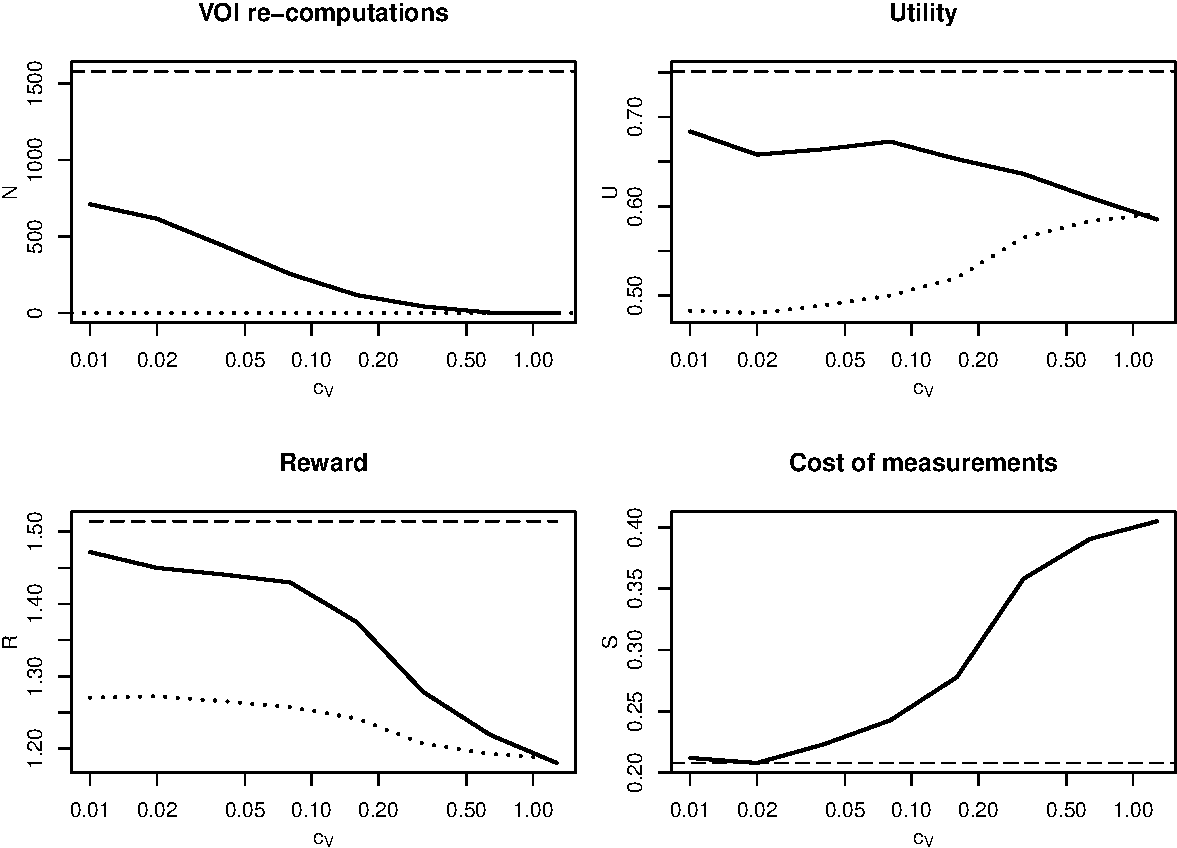
\includegraphics[scale=0.63]{ackley-myopic.pdf}
\caption{The Ackley function, myopic scheme.}
\label{fig:ackley-myopic}
\end{figure}
The Ackley function \cite{Ackley.function} is a popular optimization
benchmark. The two-argument form of the Ackley function is used in the
experiment; the function is defined by the expression (\ref{eq:emp-ackley}):
\begin{equation}
\label{eq:emp-ackley}
A(x,y)=20\cdot \exp\left(-0.2\sqrt { \frac {x^2+y^2} 2}\right)+\exp\left(\frac{cos(2\pi x)+cos(2\pi y)} 2\right)
\end{equation}
In the optimization problem, the utility function is
$u(z)=\tanh(2z)$, the measurements are normally distributed around the
true values with variance $\sigma_m^2=0.5$, and the measurement cost is
$0.01$. There are uniform dependencies with $\sigma_w^2=0.5$ in both
directions of the coordinate grid with a step of $0.2$ along each axis.
\begin{figure}[t]
\centering
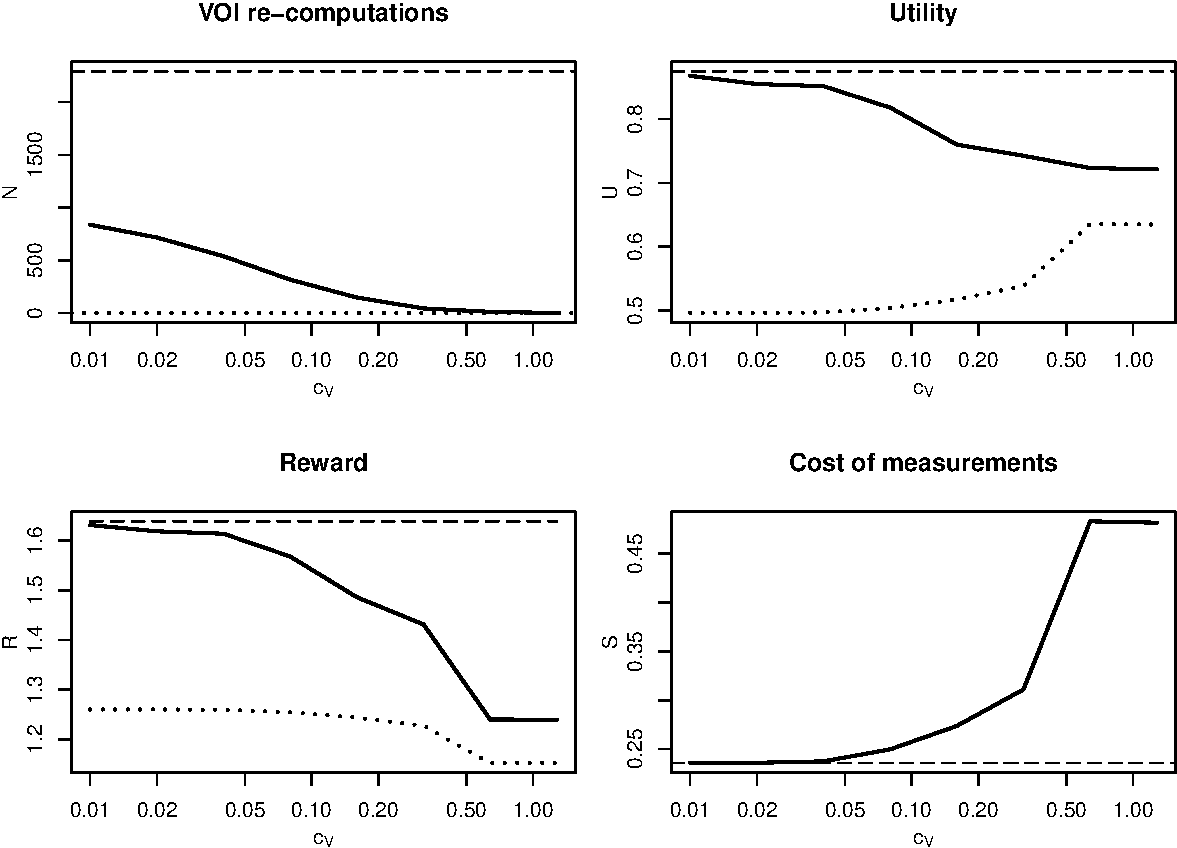
\includegraphics[scale=0.63]{ackley-blinkered.pdf}
\caption{The Ackley function, blinkered scheme.}
\label{fig:ackley-blinkered}
\end{figure}
The results are presented in Figure~\ref{fig:ackley-myopic} for the
myopic scheme, and in Figure~\ref{fig:ackley-blinkered} for the
blinkered scheme \cite{TolpinShimony.blinkered}.

\subsection{SVM Parameter Search}
\label{sec:raticomp-svm}

\begin{figure}[h]
\centering
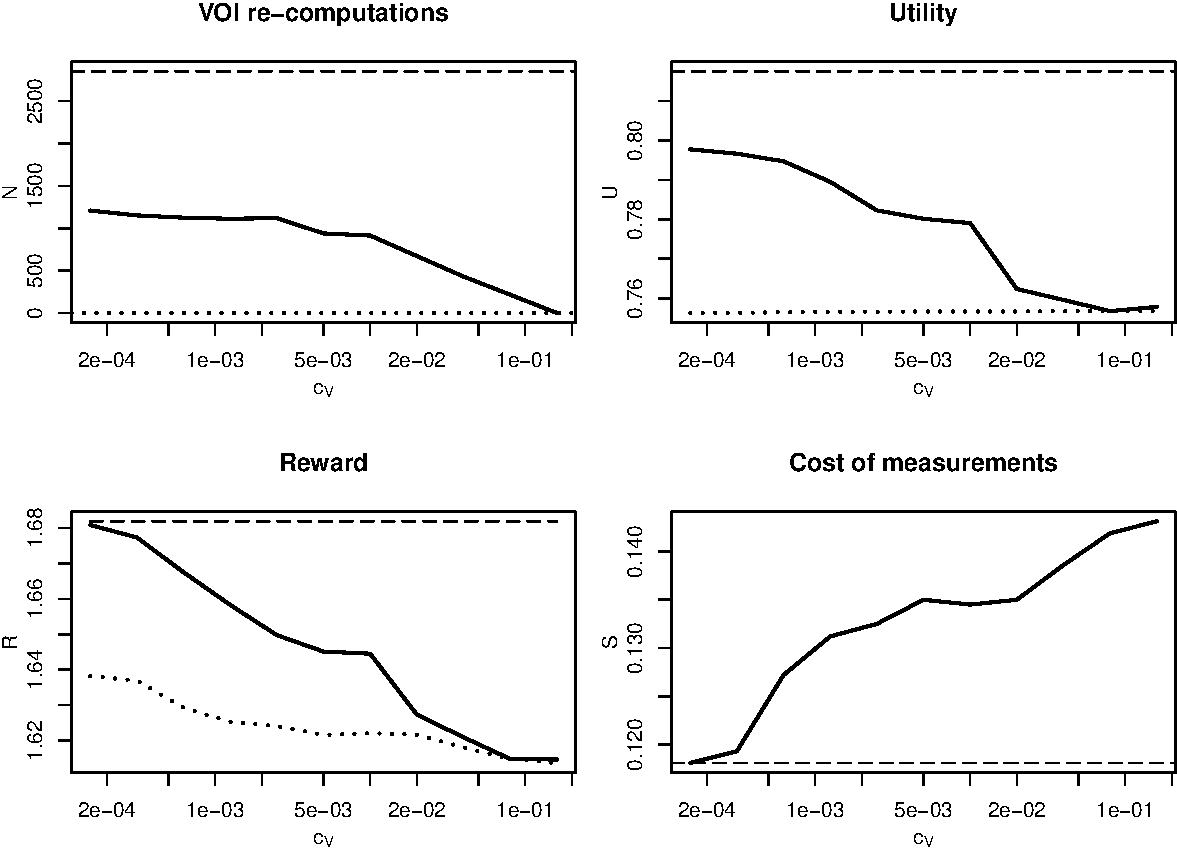
\includegraphics[scale=0.63]{svmguide2-myopic.pdf}
\caption{SVM parameter search, myopic scheme.}
\label{fig:svmguide2-myopic}
\end{figure}
An SVM (Support Vector Machine) classifier based on the radial basis
function has two parameters: $C$ and $\gamma$.  A combination of $C$
and $\gamma$ with high expected classification accuracy should be
chosen, and an efficient algorithm for determining the optimal values
is not known. A trial for a combination of parameters determines
estimated accuracy of the classifier through cross-validation. The
{\sc svmguide2} \cite{Hsu.dataset} dataset is used for the case study.
The utility function is $u(z)=\tanh(4(z-0.5))$, the $\log C$ and $\log
\gamma$ axes are scaled for uniformity to ranges $[1..21]$ and there
are uniform dependencies along both axes with $\sigma_w^2=0.4$. The
measurements are normally distributed with variance $\sigma_m^2=0.25$
around the true values, and the measurement cost is $c_m=0.01$.
\begin{figure}[h]
\centering
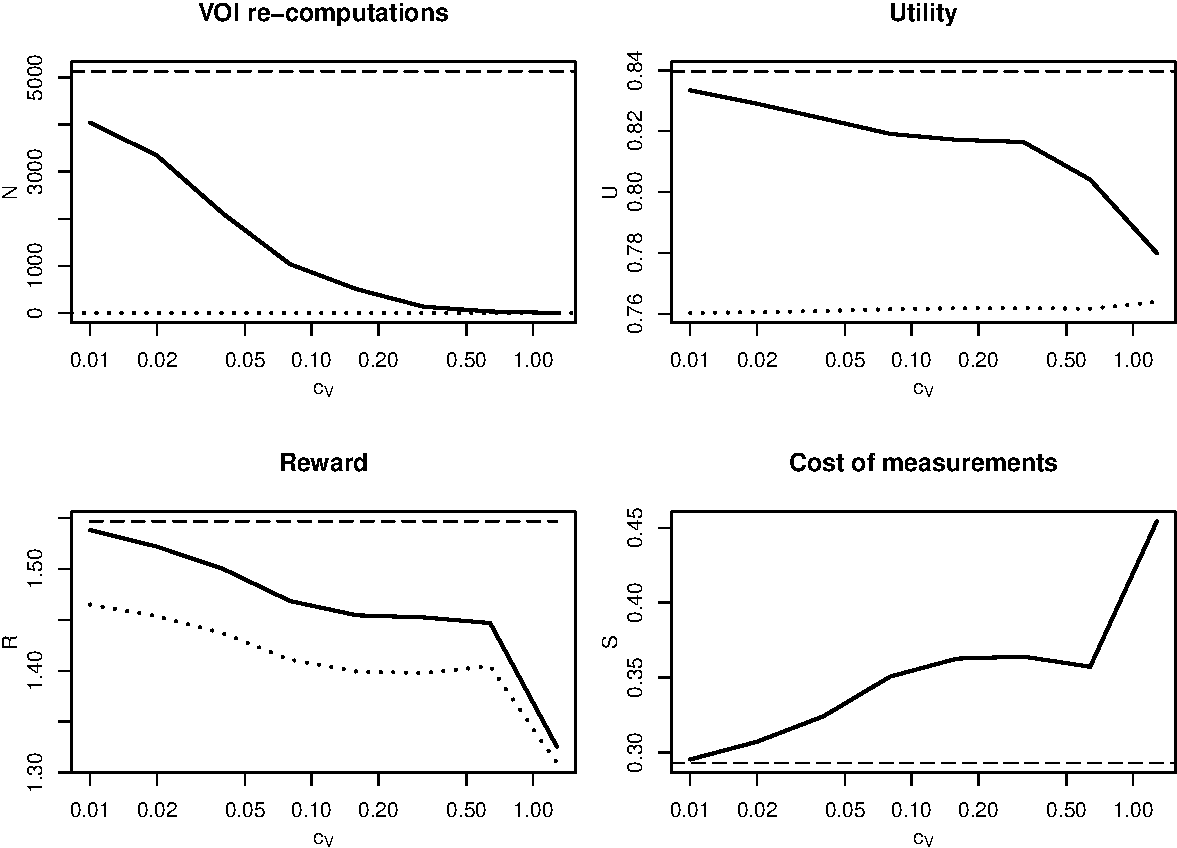
\includegraphics[scale=0.63]{svmguide2-blinkered.pdf}
\caption{SVM parameter search, blinkered scheme.}
\label{fig:svmguide2-blinkered}
\end{figure}
The results are presented in Figure~\ref{fig:svmguide2-myopic} for the
myopic scheme, and in Figure~\ref{fig:svmguide2-blinkered} for the
blinkered scheme \cite{TolpinShimony.blinkered}.

\subsection{Discussion of Results}

In all experiments, a significant decrease in computation time is
achieved with only a slight degradation of the reward; performance of
the rational recomputing algorithm decreases slowly with the
computation cost and exceeds performance of the algorithm that
makes random measurements even when VOI estimates for only a small fraction of
measurements is recomputed at each step. Exact dependency of
performance of the rational recomputing algorithm on the
overhead caused by the VOI recomputations varies among problems and depends
both on the problem properties and on the VOI estimate used in the
algorithm.

\section{Conclusion and Further Research}
\label{sec:raticomp-conclusion}

This chapter proposes an improvement to a widely used class of VOI-based
optimization algorithms. The improvement allows to decrease the
computation time while only slightly affecting the reward. The
proposed algorithm rationally reuses computations of VOI estimates and
recomputes the estimates only for measurements for which a change in
the VOI is likely to affect the choice of the next
measurement.

The proposed scheme of rational VOI computation can be further
improved.
\begin{itemize}
\item  the normal distribution is chosen rather arbitrarily to model
  uncertainty about the VOI. Often, the VOI is non-increasing
  \cite{Guestrin.submodular}, and a skewed distribution from the
  exponential family should be chosen for better results.
\item The termination condition of VOI recomputation should be
  improved such that the VOI recomputation cost could be accounted for
  in the final reward.
\item The scheme is applied to the greedy algorithm
  for measurement selection, but can be extended to other
  VOI-based algorithms.
\end{itemize}
